\chapter{Continuous Integration \& Deployment}

\includegraphics[scale=0.25]{41-about-ci-cd.jpg}

\justifying
Accommodations for Continuous Integration (CI) and Continuous Deployment (CD) in our projects directly
corresponds to our chances of success. One of the keys to a successful build pipeline is speed. Time
matters greatly as project size in terms of code base and the number of folks pushing changes grows. It
is entirely possible that your CI may take hours, or even days. What is the impact of this when you have
teams of folks pushing new changes with a high frequency? We can easily find our testing
capacity has been outstripped.

\section{GitHub Actions}

\justifying
GitHub Actions is a recent introduction to the github.com website that
lets you perform Continuous Integration on your repository, and Continuous
Deployment as desired.

\markdownInput{../labs/41-about-ci-cd/lab-41a-gh-actions.md}

\section{Linting Code in the CI Pipeline}

\justifying
There are small programs for most (every?) language that you can run before
pushing your changes to GitHub that will catch syntactical and sometimes
even programmatic issues. Consider Python, which is very sensitive with
regard to indentation. You can programatically detect and even correct issues
before your work gets too far down the pipe. This is also a good way to
make sure folks are not committing dirty code to your repositories.

\justifying
Here are some of the linters I have found useful for languages I encounter
frequently.

\begin{table}[h]
	\begin{center}
		\begin{tabular}{| p{2.5cm}| p{2.5cm} | p{2.5cm} |}
			\hline
			\textbf{Language} & \textbf{Name} & \textbf{Source}\hfill                                                        \\
			Ansible           & ansible-lint  & python (pip install ansible-lint)                                      \\
			Markdown          & mdl           & ruby (gem install mdl)                                                 \\
			Puppet            & puppet-lint   & ruby (gem install puppet-lint)\url{http://puppet-lint.com/} \\
			Python            & pylint and flake8 & python \\
		\end{tabular}
	\end{center}
\end{table}

\subsection{Docker}
\justifying
Let's see how we can leverage Actions to build the docker target in our
project. Save this YAML file under
codelab/.github/workflows/docker\_compose.yml to have GitHub Actions
execute our make docker target from our custom Makefile.

%\begin{mybox}{\thetcbcounter: A Makefile Target}
%	\lstinputlisting{code/makefile-target}
%\end{mybox}


\section{Python}
\justifying
Save this YAML file under codelab/.github/workflows/python.yml to have
GitHub Actions execute our make python target from our custom Makefile.

%\begin{mybox}{\thetcbcounter: Python GitHub action}
%	\lstinputlisting{code/makefile-target}
%\end{mybox}

\subsection{Markdown}
\justifying
The following example YAML file illustrates how to validate GitHub
flavored Markdown text files using a GitHub Action.

%\begin{mybox}{\thetcbcounter: A GitHub Action for linting markdown files}
%	\lstinputlisting{code/makefile-target}
%\end{mybox}

\justifying
Note the designation of a configuration file named .markdownlint.json at
the top level of our repository. This JSON file is used to skip certain
checks by the markdownlint tool.

%\begin{mybox}{\thetcbcounter: The .markdownlint.json config file}
%	\lstinputlisting{code/makefile-target}
%\end{mybox}

\subsubsection{Docker}

\justifying
You can test Docker containers in your CI/CD pipeline. As seen in the
following example I created a YAML file named .travis.yml to enable
automatic molecule testing of Ansible\index{Ansible} roles in Travis CI. I also set a
flag in the repo settings that prevent the PR from being merged until
Travis CI flags the build as passing.

%\begin{mybox}{\thetcbcounter: A Docker container test}
%	\lstinputlisting{code/makefile-target}
%\end{mybox}
\justifying
The contents of the requirements files and the example Ansible code is
available in the companion repo.

\subsection{Markdown}
\justifying
Save these lines to a file named .travis.yml to scan all the markdown files in your
repository.

%begin{mybox}{\thetcbcounter: A Travis config file}
%	\lstinputlisting{code/makefile-target}
%\end{mybox}

\justifying
You can also create an .mdlrc file to give mdl direction on what to scan for.

%\begin{mybox}{\thetcbcounter: A Markdown lint config file}
%	\lstinputlisting{code/makefile-target}
%\end{mybox}

\clearpage

\section{Directory Structure}

\justifying
Relevant folders and files related to our build pipeline are shown below. The users
home directory
and workspace subdirectory is implied and removed from the diagram for clarity.

\begin{figure}[!htb]
	
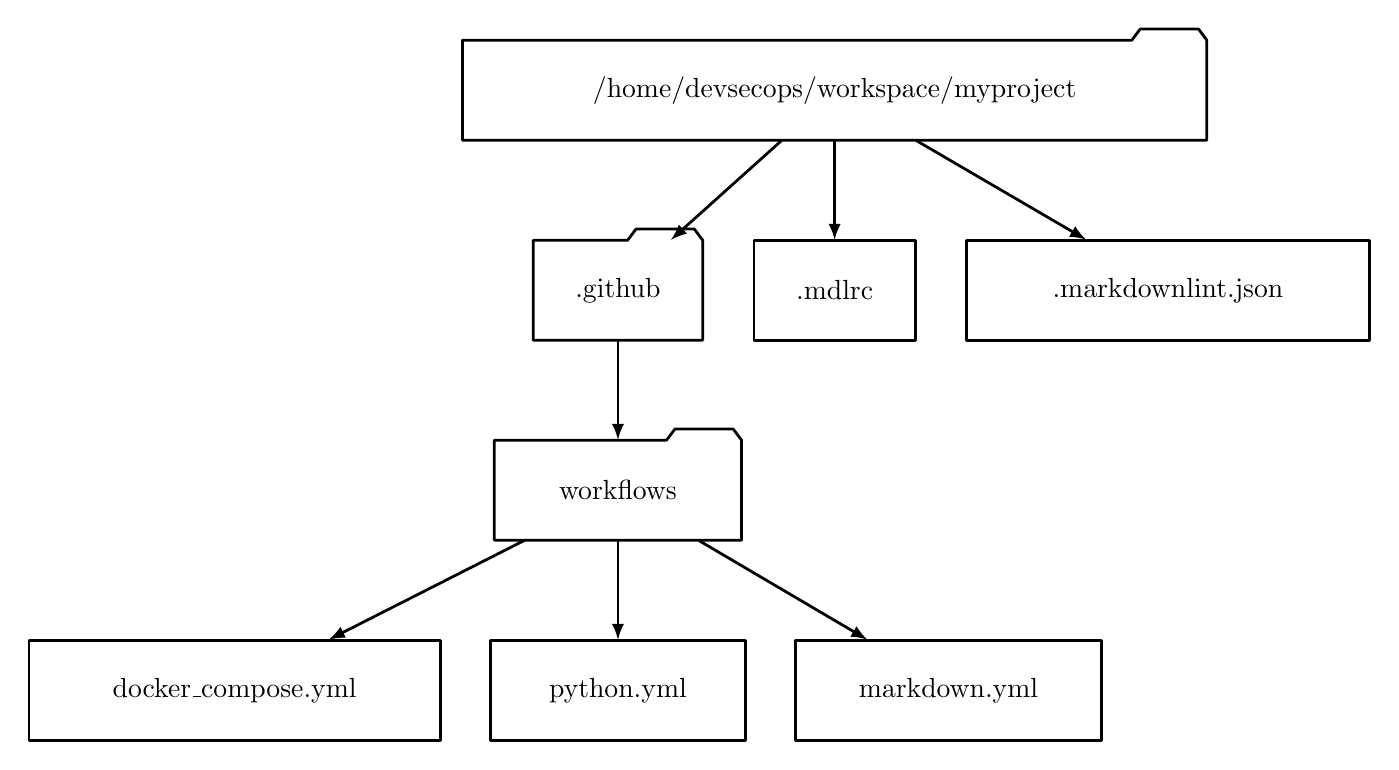
\begin{tikzpicture}[>=latex,line join=bevel,]
  \pgfsetlinewidth{1bp}
%%
\pgfsetcolor{black}
  % Edge: devsecops -> dotgh
  \draw [->] (270.72bp,215.7bp) .. controls (261.08bp,207.05bp) and (249.27bp,196.45bp)  .. (231.06bp,180.1bp);
  % Edge: devsecops -> mdlrc
  \draw [->] (290.0bp,215.7bp) .. controls (290.0bp,207.98bp) and (290.0bp,198.71bp)  .. (290.0bp,180.1bp);
  % Edge: devsecops -> mdjson
  \draw [->] (319.36bp,215.88bp) .. controls (335.05bp,206.72bp) and (354.56bp,195.34bp)  .. (380.53bp,180.19bp);
  % Edge: dotgh -> workflows
  \draw [->] (212.0bp,143.7bp) .. controls (212.0bp,135.98bp) and (212.0bp,126.71bp)  .. (212.0bp,108.1bp);
  % Edge: workflows -> dcy
  \draw [->] (178.24bp,71.876bp) .. controls (159.78bp,62.512bp) and (136.72bp,50.814bp)  .. (107.89bp,36.19bp);
  % Edge: workflows -> pyyml
  \draw [->] (212.0bp,71.697bp) .. controls (212.0bp,63.983bp) and (212.0bp,54.712bp)  .. (212.0bp,36.104bp);
  % Edge: workflows -> mdy
  \draw [->] (241.11bp,71.876bp) .. controls (256.67bp,62.724bp) and (276.02bp,51.342bp)  .. (301.78bp,36.19bp);
  % Node: devsecops
\begin{scope}
  \definecolor{strokecol}{rgb}{0.0,0.0,0.0};
  \pgfsetstrokecolor{strokecol}
  \draw (424.0bp,252.0bp) -- (421.0bp,256.0bp) -- (400.0bp,256.0bp) -- (397.0bp,252.0bp) -- (156.0bp,252.0bp) -- (156.0bp,216.0bp) -- (424.0bp,216.0bp) -- cycle;
  \draw (290.0bp,234.0bp) node {/home/devsecops/workspace/myproject};
\end{scope}
  % Node: dotgh
\begin{scope}
  \definecolor{strokecol}{rgb}{0.0,0.0,0.0};
  \pgfsetstrokecolor{strokecol}
  \draw (242.5bp,180.0bp) -- (239.5bp,184.0bp) -- (218.5bp,184.0bp) -- (215.5bp,180.0bp) -- (181.5bp,180.0bp) -- (181.5bp,144.0bp) -- (242.5bp,144.0bp) -- cycle;
  \draw (212.0bp,162.0bp) node {.github};
\end{scope}
  % Node: mdlrc
\begin{scope}
  \definecolor{strokecol}{rgb}{0.0,0.0,0.0};
  \pgfsetstrokecolor{strokecol}
  \draw (319.0bp,180.0bp) -- (261.0bp,180.0bp) -- (261.0bp,144.0bp) -- (319.0bp,144.0bp) -- cycle;
  \draw (290.0bp,162.0bp) node {.mdlrc};
\end{scope}
  % Node: mdjson
\begin{scope}
  \definecolor{strokecol}{rgb}{0.0,0.0,0.0};
  \pgfsetstrokecolor{strokecol}
  \draw (482.5bp,180.0bp) -- (337.5bp,180.0bp) -- (337.5bp,144.0bp) -- (482.5bp,144.0bp) -- cycle;
  \draw (410.0bp,162.0bp) node {.markdownlint.json};
\end{scope}
  % Node: workflows
\begin{scope}
  \definecolor{strokecol}{rgb}{0.0,0.0,0.0};
  \pgfsetstrokecolor{strokecol}
  \draw (256.5bp,108.0bp) -- (253.5bp,112.0bp) -- (232.5bp,112.0bp) -- (229.5bp,108.0bp) -- (167.5bp,108.0bp) -- (167.5bp,72.0bp) -- (256.5bp,72.0bp) -- cycle;
  \draw (212.0bp,90.0bp) node {workflows};
\end{scope}
  % Node: dcy
\begin{scope}
  \definecolor{strokecol}{rgb}{0.0,0.0,0.0};
  \pgfsetstrokecolor{strokecol}
  \draw (148.0bp,36.0bp) -- (0.0bp,36.0bp) -- (0.0bp,0.0bp) -- (148.0bp,0.0bp) -- cycle;
  \draw (74.0bp,18.0bp) node {docker\_compose.yml};
\end{scope}
  % Node: pyyml
\begin{scope}
  \definecolor{strokecol}{rgb}{0.0,0.0,0.0};
  \pgfsetstrokecolor{strokecol}
  \draw (258.0bp,36.0bp) -- (166.0bp,36.0bp) -- (166.0bp,0.0bp) -- (258.0bp,0.0bp) -- cycle;
  \draw (212.0bp,18.0bp) node {python.yml};
\end{scope}
  % Node: mdy
\begin{scope}
  \definecolor{strokecol}{rgb}{0.0,0.0,0.0};
  \pgfsetstrokecolor{strokecol}
  \draw (386.0bp,36.0bp) -- (276.0bp,36.0bp) -- (276.0bp,0.0bp) -- (386.0bp,0.0bp) -- cycle;
  \draw (331.0bp,18.0bp) node {markdown.yml};
\end{scope}
%
\end{tikzpicture}


	\caption{CI/CD related files and folders.}
\label{cicdfiles}
\end{figure}
